\documentclass[conference]{IEEEtran}
\IEEEoverridecommandlockouts
% The preceding line is only needed to identify funding in the first footnote. If that is unneeded, please comment it out.
\usepackage{cite}
\usepackage{amsmath,amssymb,amsfonts}
\usepackage{algorithmic}
\usepackage{booktabs}
\usepackage{graphicx}
\usepackage{hyperref}
\usepackage{textcomp}
\usepackage{xcolor}
\usepackage[printonlyused,withpage]{acronym}
%\usepackage{acro}
\setlength{\marginparwidth }{1.3cm}
\usepackage[colorinlistoftodos,prependcaption,textsize=tiny]{todonotes}
\def\BibTeX{{\rm B\kern-.05em{\sc i\kern-.025em b}\kern-.08em
    T\kern-.1667em\lower.7ex\hbox{E}\kern-.125emX}}

\newcommand{\itodo}[2][yellow]{\vspace{3pt}\todo[inline, color=#1!40]{#2}}
\newcommand{\mtodo}[2][orange]{\todo[color=#1!40]{#2}}

\begin{document}

\title{Between Two Worlds: Surrogate Gradients for Gradient-Based Parameter Estimation in Simplified Neuron Models}

\author{\IEEEauthorblockN{1\textsuperscript{st} Paul Mayer}
\IEEEauthorblockA{
\textit{KTH Royal Institue of Technology}\\
Stockholm, Sweden \\
pmayer@kth.se}
}

\maketitle

\itodo[green]{\textbf{REVISION SUMMARY - Priority Order:}\\
\textcolor{red}{RED = Must change (wrong framing or missing)}\\
\textcolor{cyan}{CYAN = Should improve (clarify narrative)}\\
\textcolor{orange}{ORANGE = Complete (missing content)}\\
\textcolor{blue}{BLUE = Write new section}\\
\textcolor{green}{GREEN = Suggestion/alternative}\\
\textbf{HIGH PRIORITY:}\\
1. Rewrite Introduction with new research question\\
2. Add Loss Function Design subsection (3.X) - THIS IS KEY\\
3. Write Results section with MSE failure + feature-based success\\
4. Write Discussion framing contributions honestly\\
\textbf{MEDIUM PRIORITY:}\\
5. Restructure Related Work around ``two worlds''\\
6. Complete Abstract with new framing\\
7. Update Experimental Setup with actual parameters\\
\textbf{LOW PRIORITY:}\\
8. Complete numerical integration equations\\
9. Update keywords\\
10. Fix small todos throughout
}

\begin{abstract}
  \vspace{4px}\itodo[blue]{REWRITE ABSTRACT with new framing:\\
  \textbf{Problem:} Simplified neuron models (AdEx) need parameter fitting; traditional methods use derivative-free optimization; differentiable simulators (Jaxley) enable gradient-based methods but don't support discontinuous models.\\
  \textbf{Gap:} Surrogate gradients (from SNNs) enable differentiation through spikes, but were developed for network weight training, not biophysical parameter estimation.\\
  \textbf{Contribution:} We bridge these worlds by implementing surrogate gradient-enabled AdEx in Jaxley and investigating what loss functions enable successful parameter fitting.\\
  \textbf{Finding:} MSE loss fails due to spike timing sensitivity; feature-based losses (Guarino et al.) enable optimization of bulk firing properties.\\
  \textbf{Implication:} Loss function design is critical when adapting SNN techniques for biophysical parameter estimation.}
\end{abstract}

\begin{IEEEkeywords}
Automatic Gradient Descent, Integrate-and-Fire Model, Simplified Neuron Model, Surrogate Gradients, Parameter Estimation
\end{IEEEkeywords}

\section{Introduction}\label{sec:intro}
\itodo[blue]{REWRITE INTRODUCTION - Structure it as follows:\\
\textbf{Para 1 - Context:} Neuron models need parameter fitting. Two approaches exist: (1) derivative-free methods (evolutionary algorithms) used traditionally in computational neuroscience, (2) gradient-based methods now possible with differentiable simulators like Jaxley.\\
\textbf{Para 2 - The Gap:} Jaxley works great for continuous HH-type models, but simplified models (AdEx, LIF) have discontinuous dynamics (hard reset). Surrogate gradients were developed in the SNN/ML community to handle this---but for training network weights on classification tasks, not for biophysical parameter estimation.\\
\textbf{Para 3 - Research Question:} ``Can surrogate gradient techniques be adapted for gradient-based parameter estimation of simplified neuron models? What loss function design is required?''\\
\textbf{Para 4 - Contributions:} (1) Implementation of surrogate gradient-enabled AdEx in Jaxley, (2) Investigation of loss function requirements, (3) Finding that feature-based losses work where MSE fails.\\
\textbf{Para 5 - Paper structure:} Brief roadmap.}

Ideas:
\begin{itemize}
  \item Talk about vision of simulating a whole brain (what Alex mentioned in my presentation)
  \item Say that over the last years HH were the shit, but now with the idea of simulating a whole brain simplified models have a comeback
  \item Cool innovation comes form AI ppl -> interesting mathematical concepts, they even revolutionized gpu computing
  \item Use AI tools for bio-physical simulations
\end{itemize}

\section{Background}\label{sec:background}
\subsection{Neuron Models}
Large-scale brain models are limited in size mostly by computational feasibility.
Detailed bio-physical models like the \ac{HH}-model can precisely predict membrane behaviour of a vast variety of neuron types.
However, they require huge computational resources to estimate the required parameters to fit the models to experimental data.
Simplified Neuron Models models overcome this challenge, capturing most of the sophisticated neuron behaviour with only a fraction of the computational cost, enabling large-scale simulations \cite{Gerstner2014}.
The \acf{AdEx} model \cite{Naud2008} provides a particularly interesting balance --- it reproduces a variety of firing patterns but drastically reduces the number of necessary parameters of the model.
This makes it a favourable model for large-scale neuron simulations \cite{Tesler2024}.

The \ac{AdEx} model improves the simpler \ac{LIF} model in two ways:
first, it introduces exponential behaviour when initialising the spike.
Second, the model allows for adaptation, meaning it can change spiking frequencies or post-spike refractoriness based on their firing history.
It is defined by the equations given in \cite{Brette2005, Naud2008}:
\begin{align}
  C \frac{dV}{dt} &= -g_L (V - E_L) + g_L \Delta_T \exp(\frac{V - V_T}{\Delta_T}) + I - w,\label{eq:adex1}\\
  \tau_w \frac{dw}{dt} &= a(V - E_L) - w,\label{eq:adex2}
\end{align}
with the following reset condition:
\begin{align}
  \text{if } V > 0 \text{ mV}\; \text{ then} &= \begin{cases}
    V \rightarrow V_r,\\
    w \rightarrow w_r = w + b.
  \end{cases}\label{eq:adex3}
\end{align}

It describes the membrane potential over time $V(t)$ given an injected current $I(t)$.
Equation (\ref{eq:adex1}) describes the change of potential.
$C$ is the membrane capacitance, $g_L$ the leak conductance and $E_L$ the effective resting potential.
We can understand $-g_L (V - E_L)$ as the leak current that slowly pulls the membrane potential towards it's resting potential.
$g_L \Delta_T \exp(\frac{V - V_T}{\Delta_T})$ models the depolarisation initialised by the fast reacting sodium channels using and exponential function,
modelled using a driving force based on an effective threshold potential $V_T$ and an slope factor $\Delta_T$.
$I$ is the injected current, and $w$ is the adaptation current, which is described in equation \ref{eq:adex2}.

The adaptation mechanism is controlled via an adaptation current which opposes depolarisation.
Unlike the fast membrane behaviour, this current is related to the time constant $\tau_w$, which controls the decay time.
It is controlled by $a$ (sub-threshold adaptation) as well as $b$ (spike-triggered adaptation).

Even though the number of parameters is significantly reduced compared to bio-physical \ac{HH}-type models, it still requires parameter fitting --- especially because some parameters (e.g. $a$, $b$ or $\tau_w$) do not have direct physiological counterparts (like $C$ or $g_L$).
For AdEx to perform as an effective tool, efficient methods for parameter optimizations are essential.

\subsection{Parameter Tuning for Neuron Models}
A central challenge in neuroscience has been to 'identify the parameters of detailed biophysical models, such that they match physiological measurements at scale' \cite{Deistler2025} in reasonable simulation runtimes.
The zoo of optimisation techniques is large, spanning from evolutionary algorithms \cite{VanGeit2008} to gradient descent \cite{Jones2024}, however, deciding which algorithm to use may often depend on the underlying properties of the model.
\texttt{Jaxley} \cite{Deistler2025}, a newly developed framework, uses automatic differentiation to quickly fit parameters of sophisticated biophysical models to experimental data and perform large-scale neuron simulations.
Specifically, \texttt{Jaxley} allows to simulate multi-compartment models with complex structures (dendrites, axons), cable theory equations and \ac{HH}-type ion channels.
To perform parameter optimisation, \texttt{Jaxley} uses automatic differentiation (via \texttt{Jax}).
It shows very promising results, matching or outperforming other state-of-the-art (e.g. genetic algorithms) in performance for small and large neuron models respectively.
However, as previously stated, in many circumstances it still remains unfeasible to use \ac{HH}-type models for large-scale simulations.
\texttt{Jaxley} fails to support simplified models to perform parameter tuning.
The fundamental limitation is that simplified models are not by default automatically differentiable.
This is a result of the reset condition in equation~\ref{eq:adex3}.
Addressing this issues requires special treatment: surrogate gradients.

\subsection{Surrogate Gradients}
\acfp{SG} were developed to adapt spiking neurons (usually using \ac{LIF} neuron models) for training, primarily on classification tasks.
To fit these models to real data, the typical forward pass - backward pass strategy needed to be enabled.
Because \ac{LIF}-type models have a discontinuous derivatives (see reset in equation~\ref{eq:adex3}), automatic differentiation cannot be performed without adjustments.
To overcome this issue, prior work replaced the discontinues (heavyside-) functions derivative with a (e.g. sigmoid) surrogate, but only for the backward pass \cite{Neftci2019}.
For training weights in \acp{SNN}, this performed sufficiently well.

In this work we will bridge these two worlds: combine gradient optimisation using Jaxley for using simplified models in bio-physical neuron simulations.

\section{Related Work}\label{sec:relwork}
Simplified Neuron Models historically were a necessary evil to deal with the fact that computing resources were too limited to perform large scale brain simulations with sophisticated ion-channel based models.
With the rise of cheap and widely available supercomputing, focus shifted back to more detailed \ac{HH}-type model.
In recent years however, interest in simplified models resurged, driven by mainly two reasons: researchers wanting to progress \acp{ANN} to use more detailed spiking neurons and computational neuroscientists getting closer to feasibly simulating whole mammal brains.
\subsection{Parameter Estimation for AdEx Model}
A neuron model has to replicate behaviour of a huge variety of neurons.
In simplified neuron models like \ac{AdEx}, some parameters lack a real (measurable) counterpart.
Therefore parameters have to be estimated using optimisation techniques.
Traditionally, a huge variety (from evolutionary strategies to particle swarm optimizations) of approaches were used \cite{VanGeit2008}.
A very recent paper uses grid search over a feature space, not gradients \cite{Guarino2025}.
Recently genetic algorithms, multi-state single-agent stochastic search (MSASS) or Teaching-Learning-Based Optimization (TLBO) have been used successfully to tune parameters for the \ac{AdEx} model to real voltage-clamp recordings \cite{Marin2020, Cruz2021}.
However, these approaches tend to use a lot of computational resources.

Hertag et al. \cite{Hertag2011} developed an analytical approximation to the AdEx model to speed up computations.
Using automatic differentiation could also address this issue.
Jones et al. \cite{Jones2024} and Deistler2025 et al. \cite{Deistler2025} demonstrated that gradient-based methods can effectively parametrize HH-type models.
However, they require the inherently differentiable nature of HH-type models.
Simplified models require additional treatment to benefit from this technique.

\subsection{Parameter Learning using Surrogate Gradients in Spiking Neural Networks}
Previous work explored using surrogate gradients for training weights of \acp{SNN} in classification tasks \cite{Neftci2019, Gerum2021, Perez-Nieves2021}.
Gerum and Schilling \cite{Gerum2021} explored different surrogates (like sigmoid or esser function) to train a \ac{LIF} based \ac{NN} for image classification tasks.
The authors used \texttt{Keras} to perform automatic differentiation and backpropagation.
Perez-Nieves et al. \cite{Perez-Nieves2021} used a sigmoidal surrogate gradient in the backward pass to train a spiking NN in \texttt{PyTorch} to perform a variety of different classification tasks.
However, their work focuses on training network weights on task-based classification tasks.

Recent theoretical work \cite{Gygax2025} clarifies why surrogate gradients succeed despite approximating the true gradient.
But fitting biophysical parameters to experimental recordings poses a different challenge:
the loss function must quantify similarity between simulated and recorded spike trains.
Whether standard choices like mean squared error suffice --- 
or whether domain-specific alternatives are required --- 
remains unexplored.
This work investigates this question.

\subsection{Benchmark Sets for Neuron Models}
Neuron models are highly specialised and are fit to very specific data.
Therefore it proves to be difficult to compare models systematically.
Jolivet et al. \cite{Jolivet2008} introduce a coincidence factor, which allows to evaluate neuron models.
We use the concept to evaluate the quality of trained parameters 

This work will try to replicate the model behaviour given by existing implementations \cite{Stimberg2019} using the parameters given by \cite{Naud2008}.
For benchmarking the optimisation behaviour, we will fit the model use voltage traces of \acp{SPN} gained from experiments by Johansson et al. \cite{Johansson2020}.

\section{Methodology}\label{sec:method}
This work introduces two contributions: firstly, we implement the \ac{AdEx} model within \texttt{Jaxley}, providing both standard and surrogate gradient variants.
The surrogate implementation can easily adopted to Jaxleys existing simplified models: \ac{LIF} and Izhikevich.
Secondly, we use \texttt{Jaxley} to perform gradient-based optimisation.
We investigate two different loss functions:
\begin{itemize}
  \item \ac{MSE}
  \item Guarino et al. \cite{Guarino2025} feature-based loss function.
\end{itemize}
Using gradient-based optimisation requires a differentiable loss function.
Therefore we will introduce a gradient version of the feature-based loss function.

\subsection{Integration of Surrogate Gradients into Jaxley}
\texttt{Jaxley} is built on top of \texttt{JAX} and leverages its automatic differentiation capabilities for gradient-based parameter optimisation.
Neuron dynamics in \texttt{Jaxley} are defined through \texttt{Channel} classes, which specify three core methods: \texttt{update\_states()} for state variable evolution, \texttt{compute\_current()} for membrane current contributions, and \texttt{init\_state()} for initialisation of state variables.
During simulation, \texttt{JAX} traces these functions to construct a computational graph, enabling automatic gradient computation and backpropagation.

\subsubsection{The Differentiability Problem}
Simplified neuron models employ a discrete reset mechanism when the membrane potential crosses a threshold.
This reset is mathematically expressed using the Heavyside step function $H$:
\begin{equation}
    H(v - v_{\text{th}}) = \begin{cases} 1 & \text{if } v \geq v_{\text{th}} \\ 0 & \text{otherwise} \end{cases}
\end{equation}
The derivative of the Heavyside function is zero almost everywhere (and undefined at the threshold):
\begin{equation}
    \frac{\partial H}{\partial v} = 0 \quad \text{for } v \neq v_{\text{th}}
\end{equation}
This causes gradients to vanish during back-propagation through spike events, which prevents gradient-based optimisation from working.

\subsubsection{Surrogate Gradient Approach}
To overcome this limitation, we employ surrogate gradients \cite{Neftci2019}: the forward pass uses the original Heavyside function to maintain correct spike dynamics, while the backward pass substitutes the function with a surrogate.
This is implemented in \texttt{JAX} using \texttt{jax.custom\_vjp}, which allows defining custom vector-Jacobian products.

We implement three surrogate gradient functions, each providing different gradient characteristics:

\textbf{Sigmoid surrogate:}
\begin{equation}
    \frac{\partial \tilde{H}}{\partial x} = \beta \cdot \sigma(\beta x) \cdot (1 - \sigma(\beta x))
\end{equation}
where $\sigma$ is the sigmoid function and $\beta$ controls the steepness.

\textbf{Exponential surrogate:}
\begin{equation}
    \frac{\partial \tilde{H}}{\partial x} = \beta \cdot \exp(-\beta |x|)
\end{equation}

\textbf{SuperSpike surrogate} \cite{Zenke2018}:
\begin{equation}
    \frac{\partial \tilde{H}}{\partial x} = \frac{1}{(\beta |x| + 1)^2}
\end{equation}

All three surrogates are centred at the threshold ($x = v - v_{\text{th}}$).
The hyperparameter $\beta$ controls the sharpness: higher values produce steeper gradients at the threshold, while lower values spread the gradient over a wider voltage ranges.

\subsubsection{Implementation Details}
We reformulate the conditional reset from a discrete selection:
\begin{equation}
    v_{\text{new}} = \begin{cases} v_{\text{reset}} & \text{if spike} \\ v & \text{otherwise} \end{cases}
\end{equation}
to a continuous, differentiable form:
\begin{equation}
    v_{\text{new}} = s \cdot v_{\text{reset}} + (1 - s) \cdot v
\end{equation}
where $s = \tilde{H}(v - v_{\text{th}})$ is the surrogate spike indicator, to ensure differentiability through the reset mechanism.
This formulation allows gradients to flow through the reset operation.

This approach can easily be applied to the existing \ac{LIF} (\texttt{Fire\-Surrogate}) and Izhikevich models in \texttt{Jax\-ley},
not only to the newly implemented \ac{AdEx} model (\texttt{AdEx\-Surro\-gate}).

\subsection{AdEx Model Implementation}\label{sec:adex_impl}
We implement the \ac{AdEx} model as a \texttt{Jaxley} channel, following the formulation by Brette and Gerstner \cite{Brette2005} (see Equations~\ref{eq:adex1}--\ref{eq:adex3}).
Unlike \ac{HH}-type channels that contribute currents to a shared voltage solver, simplified models like \ac{AdEx} handle voltage integration directly within their \texttt{update\_states()} method.
We follow the implementation pattern of \cite{Deistler2025}.

\subsubsection{Numerical Integration}
The \ac{AdEx} model consists of two coupled differential equations requiring different numerical treatment:

\textbf{Adaptation current $w$:}
Equation~\ref{eq:adex2} is a linear dynamic system in $w$, allowing the use of exponential Euler integration.
It has the analytical solution
\begin{equation}
  w(t+\Delta t) = w(t) \cdot e^{-\Delta t / \tau_w} + a(V - E_L)(1 - e^{-\Delta t / \tau_w})
\end{equation}\label{eq:adaption-current-integration}
which gives increased numerical stability compared to e.g. forward euler methods.

\textbf{Membrane potential $V$:}
The exponential term in Equation~\ref{eq:adex1} makes this equation nonlinear, requiring forward Euler integration:
\begin{equation}
    V(t + \Delta t) = V(t) + \Delta t \cdot \frac{dV}{dt}
\end{equation}
To prevent numerical overflow from the exponential spike mechanism, we clamp the argument:
\begin{equation}
    \exp\left(\frac{V - V_T}{\Delta_T}\right) \rightarrow \exp\left(\min\left(\frac{V - V_T}{\Delta_T}, 10\right)\right)
\end{equation}

\subsubsection{Spike Detection and Reset}
After each integration step, we check for threshold crossing ($V > v_{\text{threshold}}$).
If the threshold is crossed, we apply the reset conditions from Equation~\ref{eq:adex3}.
For standard \texttt{LIF}, \texttt{AdEx} or \texttt{Izhikevich}, this uses \texttt{jax.lax.select()} for conditional assignment.
In the differentiable variants, we use the continuous formulation described in Section~\ref{sec:method} for both $V$ and $w$:
\begin{align}
    V_{\text{new}} &= s \cdot V_r + (1 - s) \cdot V, \\
    w_{\text{new}} &= s \cdot (w + b) + (1 - s) \cdot w,
\end{align}
where $s: V\rightarrow [0,1]$ is the surrogate of the heavyside function.

\subsubsection{Model Parameters}
Table~\ref{tab:adex_params} summarises the \ac{AdEx} parameters and their default values.
Parameters without direct physiological counterparts (e.g., $a$, $b$, $\tau_w$) are primary targets for optimisation.

\begin{table}[t]
\centering
\caption{\ac{AdEx} model parameters and default values.}
\label{tab:adex_params}
\begin{tabular}{llll}
\toprule
\textbf{Parameter} & \textbf{Symbol} & \textbf{Default} & \textbf{Unit} \\
\midrule
Membrane capacitance & $C$ & 200 & pF \\
Leak conductance & $g_L$ & 10 & nS \\
Leak reversal & $E_L$ & -70 & mV \\
Threshold potential & $V_T$ & -50 & mV \\
Slope factor & $\Delta_T$ & 2 & mV \\
Reset potential & $V_r$ & -58 & mV \\
Detection threshold & $v_{\text{threshold}}$ & 0 & mV \\
Adaptation time constant & $\tau_w$ & 30 & ms \\
Subthreshold adaptation & $a$ & 2 & nS \\
Spike-triggered adaptation & $b$ & 0 & pA \\
Stimulation current & $I$ & 500 & pA\\
\bottomrule
\end{tabular}
\end{table}

AdEx is defined using absolute capacitance ($pF$).
However, Jaxley is targeted at bio-physical HH-type simulations, and therefore works with cell morphology and gemoetries.
It therefore expects specific capacitance ($\mu F/cm^2$).
To circumvent this problem, we compute a fictitious cylindrical geometries whose surface area yields the desired total capacitance assuming jaxleys standard specific capacitance ($1 \mu F/cm^2$).
This scales injected currents to maintain correct dynamics.

\subsection{Implementation Verification}\label{sec:verification}
\begin{figure*}
  \begin{center}
    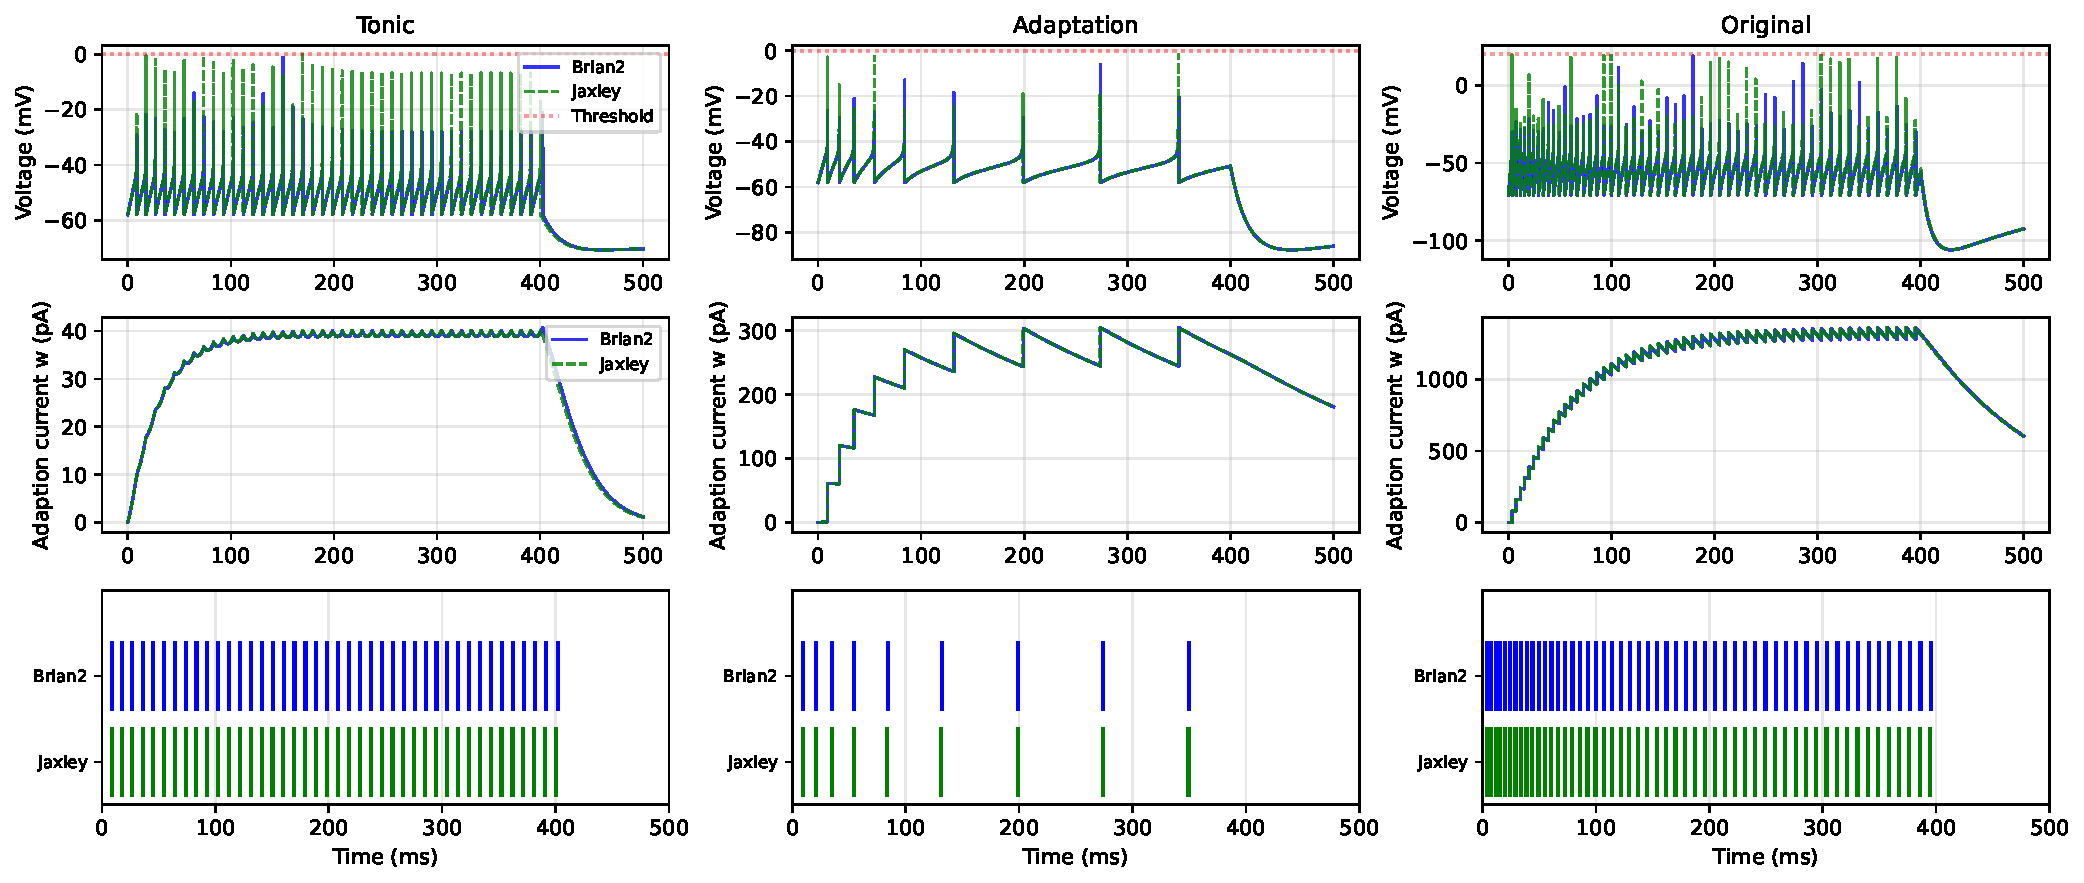
\includegraphics[width=\textwidth]{figures/adex_comparison_combined.pdf}
  \end{center}
  \caption{Left to right: tonic, adaption and original parameters.
Tonic and adaption parameters refer to the parameters provided by \cite{Naud2008}, original parameters are the parameters used in the original AdEx paper \cite{Brette2005}.
Top row shows the simulated voltage traces.
Interesting to note is that when the threshold is reached, the voltage is reset in the same time step.
This leads to the voltage never crossing the threshold line in the recordings.
Second row displays the adaption current $w$.
Last row compares the spike timings between \texttt{Brian2} and \texttt{Jaxley}.
We expect minor numerical differences, mainly to the fact that different integration methods are used.}\label{fig:brian_comparison}
\end{figure*}

To verify the correctness of our \ac{AdEx} implementation, we compare simulation outputs against Brian2 \cite{Stimberg2019}, a widely-used reference simulator for spiking neural networks.

\subsubsection{Comparison Setup}
Both simulators are configured identically:
\begin{itemize}
    \item Time step: $\Delta t = 0.01$ ms
    \item Simulation duration: 500 ms
    \item Stimulation duration: 400 ms
    \item Initial conditions: $V(0) = V_r$, $w(0) = 0$
\end{itemize}

\subsubsection{Test Cases}
We evaluate three parameter configurations from Naud et al.\ \cite{Naud2008} that produce distinct firing patterns:

\textbf{Tonic spiking}:\\
Regular spiking without spike-frequency adaptation, serving as a baseline case.
The parameters are the default parameters (see \ref{tab:adex_params}).

\textbf{Adaptation}:\\
Strong spike-triggered adaptation with slow decay, producing decreasing firing rates over time.
The parameters used are
$C_m = 200$,
$g_L = 12$,
$E_L = -70$,
$v_T = -50$,
$\Delta_T = 2$,
$v_r = -58$,
$v_{\text{threshold}} = 0$,
$\tau_w = 300$,
$a = 2$,
$b = 60$,
$I = 500$.

\textbf{Original parameters} \cite{Brette2005}:\\
The original parameter set from Brette and Gerstner, demonstrating combined adaptation mechanisms.
The parameters used are
$C_m = 281$,
$g_L = 30$,
$E_L = -70.6$,
$v_T = -50.4$,
$\Delta_T = 2$,
$v_r = -70.6$,
$v_{\text{threshold}} = 20$,
$\tau_w = 144$,
$a = 4$,
$b = 80.5$,
$I = 2500$.

\subsubsection{Comparison Metrics}
We assess implementation correctness through:
\begin{itemize}
  \item \textbf{Visual comparison:} Overlay of voltage traces from both simulators (Figure~\ref{fig:brian_comparison}).
  \item \textbf{Spike count:} Both implementations produce identical spike counts for all test configurations.
  \item \textbf{Spike timing:} Maximum absolute difference in spike times $\max_i |t_i^{\text{Jaxley}} - t_i^{\text{Brian2}}| < 1$ ms.
\end{itemize}

\subsection{Parameter Optimisation Evaluation}\label{sec:param_opt}
To evaluate the effectiveness of gradient-based optimisation with surrogate gradients, we fit \ac{AdEx} model parameters to experimental voltage recordings.

As training data, we used voltage recordings from mouse striatal neurons given by \cite{Johansson2020}.
For now we only used a single recording. 
\footnote{The data can be found in the cell folder \texttt{mCP-dspn-e150917\_c\-6\_D1-manimal\_1\_n24\_04102017\_cel1/}\texttt{ECBL\_IDthresh\_ch\-4\_553.dat} (stimulation) and
\texttt{ECBL\_IDthresh\_ch5\_553.dat} (cell response)}

As simulation parameters we used \itodo[red]{important: finish this}

%  - Time step (dt): inferred from experimental data (~0.1 ms typical for such recordings)
%  - Maximum training window: 500 ms (max_duration_ms = 500.0)
%  - Total simulation duration: stim_duration_ms + 100 ms (includes post-stimulus period)
%  - Surrogate gradient: sigmoid with slope = 25.0
%
%  Training Setup
%
%  - Optimizer: Adam (via Optax)
%  - Learning rate: 0.1
%  - Epochs: 500
%  - Gradient clipping: global norm clipping with max norm = 2.0
%  - Early stopping: best parameters checkpointed based on lowest loss
%  - NaN handling: gradient updates skipped when NaN detected
%
%  Trainable vs Fixed Parameters
%  ┌──────────────────────────────────┬───────────────────────────────────┐
%  │            Trainable             │               Fixed               │
%  ├──────────────────────────────────┼───────────────────────────────────┤
%  │ g_L (leak conductance)           │ C_m (membrane capacitance)        │
%  ├──────────────────────────────────┼───────────────────────────────────┤
%  │ E_L (leak reversal)              │ delta_T (spike slope factor)      │
%  ├──────────────────────────────────┼───────────────────────────────────┤
%  │ v_T (spike threshold)            │ v_threshold (detection threshold) │
%  ├──────────────────────────────────┼───────────────────────────────────┤
%  │ v_reset (reset potential)        │ radius, length (geometry)         │
%  ├──────────────────────────────────┼───────────────────────────────────┤
%  │ tau_w (adaptation time constant) │                                   │
%  ├──────────────────────────────────┼───────────────────────────────────┤
%  │ a (subthreshold adaptation)      │                                   │
%  ├──────────────────────────────────┼───────────────────────────────────┤
%  │ b (spike-triggered adaptation)   │                                   │
%  └──────────────────────────────────┴───────────────────────────────────┘

\subsubsection{Dataset}
We use intracellular recordings from striatal projection neurons provided by Johansson and Silberberg \cite{Johansson2020}.
The dataset contains voltage traces from four distinct striatal neuron types, recorded under current-clamp conditions.
\mtodo{Specify which 4 neuron types once data is confirmed}

\subsubsection{Optimisation Setup}
We optimise a subset of \ac{AdEx} parameters that lack direct physiological measurements: $\{a, b, \tau_w, V_T, \Delta_T\}$.\mtodo[red]{Fix this! This is wrong.}
Parameters with known physiological values ($C$, $g_L$, $E_L$) are fixed based on experimental measurements where available.

\subsection{Loss Function}\mtodo[orange]{Should this be a subsection or subsubsection?}
\subsubsection{MSE}
The \ac{MSE}-Loss is defined as 
\begin{equation}\label{eq:MSE}
    \mathcal{L}_{\text{MSE}}(\theta) = \frac{1}{T} \sum_{t=1}^{T} \left( V_{\text{sim}}(t; \theta) - V_{\text{exp}}(t) \right)^2,
\end{equation}
where $\theta$ denotes the trainable parameters.

\itodo[blue]{write MSE section}
\begin{itemize}
  \item MSE on voltage traces seems natural but fails for spiking neurons
  \item  Problem: small timing differences create huge MSE even if spike patterns are similar
  \item The loss landscape is non-convex; gradients don't point toward good solutions
  \item Show equation, explain why it fails
\end{itemize}
\subsubsection{Feature-Based Loss}
\itodo[blue]{write feature-based loss section}
\begin{itemize}
  \item Alternative: extract electrophysiological features, compare features instead of traces
  \item Based on Guarino et al. cite
  \item Features: spike timing (t\_first, t\_second, t\_last), ISI (inverse first/last ISI), firing frequency, v\_stim\_end
  \item Loss = weighted sum of relative errors: $|f_{sim} - f_{exp}| / |f_{exp}|$
  \item Missing feature penalty: if exp has spike but sim doesn't, add penalty
\end{itemize}
\subsubsection{Differentiable Feature-Based Loss}
\itodo[blue]{write feature-based loss section}
\begin{itemize}
  \item Challenge: feature extraction typically uses hard thresholds (non-differentiable)
  \item Our contribution: soft/differentiable versions of all features
  \item Soft spike count using surrogate spike indicator
  \item Soft spike timing using weighted time averages
  \item Temperature parameter controls sharpness vs gradient trade-off
\end{itemize}
\subsubsection{Multi-Trace Loss}
\itodo[blue]{write feature-based loss section}
\begin{itemize}
  \item Single trace: many parameter combinations can produce similar output
  \item Multi-trace: same parameters must match across different current injection levels
  \item Provides much stronger constraints, better generalization
\end{itemize}

\mtodo[red]{DELETE these old todos, replace with new structure above}
\mtodo{Consider spike-timing based loss as alternative, I even assume this is way to go.}
\mtodo{Check what other ppl are doing}

\textbf{Optimiser:} Adam optimiser with learning rate $\eta$.
\mtodo{Specify learning rate and number of iterations after experiments}

\textbf{Initialisation:} Parameters are initialised within physiologically plausible ranges based on literature values \cite{Naud2008}.

\itodo[blue]{Differentiable Guarino et al.}
Guarino et al. \cite{Guarino2025},

\subsubsection{Evaluation Metrics}
We assess optimisation performance through:
\begin{itemize}
    \item Final loss value (voltage trace MSE)
    \item Visual comparison of fitted vs.\ experimental traces
    \item Spike timing accuracy (if applicable)
    \item Convergence behaviour (loss vs.\ iteration)
\end{itemize}
\itodo[blue]{ADD: Coincidence Factor $\Gamma$ (Jolivet et al. 2008) as quantitative evaluation metric:\\
\textbf{3.X.Y Coincidence Factor for Spike Train Evaluation}\\
- The coincidence factor $\Gamma$ measures spike timing prediction quality, normalized by chance level\\
- Formula: $\Gamma = \frac{N_{coinc} - \langle N_{coinc} \rangle}{0.5(N_{data} + N_{model})} \cdot \frac{1}{1 - 2f\Delta}$\\
- $N_{coinc}$: coincidences within $\pm\Delta$ (default 2ms), $f$: model firing rate\\
- $\Gamma = 1$: perfect prediction, $\Gamma = 0$: chance level, $\Gamma < 0$: worse than chance\\
- Reference values from Jolivet et al.: well-fitted aEIF achieves $\Gamma_A \approx 0.82-0.83$\\
- Use to compare: (1) our fitted parameters vs (2) well-fitted reference parameters\\
- Implementation complete in \texttt{coincidence\_factor.py}}


\mtodo[green]{REFRAME: You're not comparing \emph{against} Guarino as baseline.
You're \emph{adapting} their feature-based approach for gradient-based optimization.
The comparison is MSE vs feature-based, not your method vs Guarino's grid search.}

\section{Experimental Setup}\label{sec:expsetup}
All experiments were conducted on a 2020 Apple Silicon Mac.
Software is written in python and executed using python version 3.14.2.
The implementation is built on Jaxley version 0.12.0.
Comparison were performed using the Brian2 simulator 2.10.1.
Full list of software versions is found in the \href{https://github.com/paulmyr/DD2375-HT25-Project-Course-in-High-Performance-Computing/blob/master/requirements.txt}{requirements.txt}

\section{Results}\label{sec:results}
\subsection{AdEx verification}
Running verification\footnote{Test can be run in \href{https://colab.research.google.com/github/paulmyr/DD2375-HT25-Project-Course-in-High-Performance-Computing/blob/master/5_evaluation/notebooks/jaxley_test_adex.ipynb}{Google Colab}} against \texttt{Brian2} gave the following results:
Figure~\ref{fig:brian_comparison} demonstrates almost perfect overlap.
The biggest differences are in spike magnitude.
We note that both brian2 and jaxley results do not cross the detection threshold in the recording.
This is an artefact due to how we record the simulated potentials.
The integration step is computed and then the new voltage value is stored.
When the integrated value crosses the threshold, the voltages are reset before the value is recorded, meaning in this all voltage recordings are below $v_{\text{threshold}}$.

We measured the difference between spike timings.
Table~\ref{tab:spike_comparison} shows the measured results.
We identify over different spiking behaviour, both simulations produced identical amount of spikes.
The measured maximum timing differences between spikes was $<1$ms for all runs, the mean difference between spikes was $<0.5ms$.
Given the sensitivity of the exponential spiking initiation zone and the fact that different numerical integration was used for the adaption current,
we were satisfied with the similarity of the results and concluded that the implementation is correct.

\begin{table}[t]
\centering
\caption{Spike timing comparison between Jaxley and Brian2 implementations.}
\label{tab:spike_comparison}
\begin{tabular}{lccc}
\toprule
 & Tonic & Adaptation & Original \\
\midrule
Spike count & 52 & 10 & 64 \\
Max timing diff.\ (ms) & 0.54 & 0.58 & 0.82 \\
Mean timing diff.\ (ms) & 0.28 & 0.27 & 0.42 \\
\bottomrule
\end{tabular}
\end{table}

\subsection{Surrogate Gradient verification}
To verify the surrogate gradient implementation we first computed the gradient of a simple loss function (number of spikes) after stimulating the cell.
The produced gradients are zero for the default implementation and non-zero for the surrogate model.
We visualized (see figure~\ref{fig:surrogate_gradients_comparison}) the backward pass to verify compare different surrogate types (Sigmoid, Exponential, SuperSpike) --- all peak around threshold of the heavyside-function.

\begin{figure}[t]
  \begin{center}
    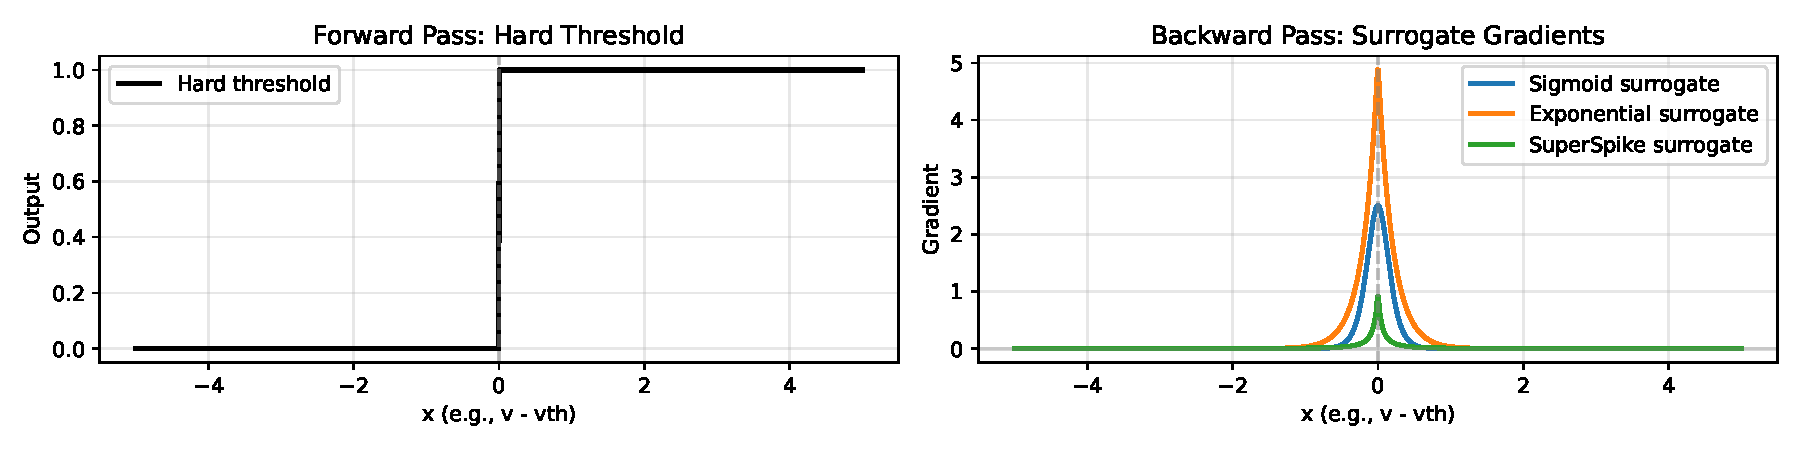
\includegraphics[width=\columnwidth]{figures/surrogate_gradients_comparison.pdf}
  \end{center}
  \caption{Left: heavyside function in the forward pass. Right: different surrogate gradients, all centred around the threshold.}\label{fig:surrogate_gradients_comparison}
\end{figure}

\subsection{Parameter Estimation using MSE}
  The natural first approach for parameter estimation is to minimize the \ac{MSE}\ref{eq:MSE} between simulated and experimental voltage traces.
  However, our experiments indicated that this loss function is fundamentally unsuitable for spiking neurons.
  A core problem is \emph{spike timing sensitivity}: even when simulated and experimental traces exhibit similar firing patterns, small temporal misalignments between spikes create disproportionately large MSE values.
  Consider two traces with identical spike counts and frequencies, but with spikes offset by 2\,ms.
  During each spike, the voltage difference can exceed 100\,mV (from resting potential to spike peak), resulting in enormous per-sample errors that dominate the loss.
  This timing sensitivity manifests in a highly non-convex loss landscape.
  The gradient at any point reflects primarily the instantaneous voltage mismatch rather than structural similarity of the spike trains.
  Consequently, gradient descent steps often move parameters in directions that reduce voltage error at specific time points while disrupting the overall firing pattern.

  Additionally, perfekt spike time matchings are punished.
  This is because \ac{AdEx} values are reset before the jaxley simulator records the voltage trace --- if experimental data and simulation data would spike at the exact same time, 
  the loss would be huge (AdEx is at $V_{r}$, experiment is at $V_{\text{peak}}$).
  This enforces a mismatch between spike timing and simulation.

  We attempted MSE-based optimization using the same experimental recordings and training setup described in Section~\ref{sec:param_opt}.
  The optimizer converged to parameter configurations that minimized voltage deviation during subthreshold periods but failed to produce correct spiking behaviour.
  In many runs, the model either stopped spiking entirely (eliminating spike-related MSE contributions) or produced spike patterns uncorrelated with the experimental data.

  This leads us to believe that MSE loss, while theoretically sound for continuous signals, is ill-suited for discrete event (spike) matching.
  The loss function must capture \emph{what} features matter rather than demanding exact sample-by-sample voltage alignment.

\subsection{Parameter Estimation using Feature-Based Loss}
\subsection{Coincidence Factor}
To evaluate the performance of the two loss functions, we simulated 

We evaluated spike timing prediction quality using the coincidence factor $\Gamma$ from Jolivet et al.~\cite{Jolivet2008}, with coincidence window $\Delta = 2$\,ms.
Table~\ref{tab:coincidence} compares different parameter configurations.

\begin{table}[t]
\centering
\caption{Coincidence factor $\Gamma$ for different parameter sets. Reference: well-fitted aEIF achieves $\Gamma \approx 0.82$--$0.83$~\cite{Jolivet2008}.}
\label{tab:coincidence}
\begin{tabular}{lcccc}
\toprule
\textbf{Parameters} & $\Gamma$ & $N_{\text{coinc}}$ & $N_{\text{exp}}$ & $N_{\text{sim}}$ \\
\midrule
Initial (untrained) & --- & --- & --- & --- \\
MSE loss & --- & --- & --- & --- \\
Guarino loss & --- & --- & --- & --- \\
\bottomrule
\end{tabular}
\end{table}
\mtodo{Run evaluate\_coincidence.py and fill in actual values}

\mtodo{Add bar chart figure comparing $\Gamma$ values with reference lines at 0.82 (well-fitted) and 0 (chance)}

The trained parameters achieved $\Gamma = XXX$, indicating [GOOD/MODERATE/POOR] spike timing prediction compared to the Jolivet et al.\ benchmark of $\Gamma \approx 0.82$ for well-fitted models.
\subsection{Summary}

\itodo[blue]{RESULTS - Structure as follows:\\
\textbf{5.2 Gradient Flow Verification}\\
- Reference your test\_guarino\_features.py results (all 7 tests pass)\\
- This proves surrogate gradients work in this context\\
\textbf{5.3 MSE Loss Failure}\\
- Show training with MSE doesn't converge / converges to wrong solution\\
- Visualize: loss curve, final voltage trace comparison\\
- Explain why: timing sensitivity, non-convex landscape\\
\textbf{5.4 Feature-Based Loss Success}\\
- Show training with Guarino features works\\
- Your results: spike count matches (13 vs 13), firing freq matches (26 Hz)\\
- Limitation: spike timing still needs tuning (35ms vs 22ms)\\
- Multi-trace results if available\\
\textbf{5.5 Quantitative Summary}\\
- Table comparing MSE vs Feature-based on key metrics\\
- Spike count error, frequency error, timing error\\
\textbf{5.6 Coincidence Factor Evaluation}\\
- Report $\Gamma$ values for fitted parameters vs experimental data\\
- Compare against reference: well-fitted aEIF achieves $\Gamma_A \approx 0.82-0.83$\\
- Use $\Delta = 2$ms coincidence window (standard from Jolivet et al.)}

\section{Discussion and Conclusion}\label{sec:discussion}
\itodo[blue]{DISCUSSION - Structure as follows:\\
\textbf{6.1 Key Findings}\\
- Surrogate gradients successfully enable differentiation through spikes\\
- MSE loss is fundamentally unsuitable for spike train matching\\
- Feature-based loss enables optimization of bulk firing properties\\
- Spike timing precision remains challenging\\
\textbf{6.2 Implications}\\
- Loss function design is critical when bridging SNN techniques to biophysical fitting\\
- Can't just transfer SNN methods directly; need domain-specific adaptations\\
- Feature-based losses from computational neuroscience (Guarino, eFEL) are key\\
\textbf{6.3 Limitations}\\
- Spike timing not perfectly matched (honest about this)\\
- Single neuron type tested\\
- No runtime comparison (because convergence is the primary concern)\\
\textbf{6.4 Future Work}\\
- Better spike timing losses\\
- More neuron types\\
- Comparison with evolutionary methods once optimization is reliable\\
\textbf{6.5 Conclusion}\\
- We bridged two worlds: SNN surrogate gradients + biophysical parameter fitting\\
- Key insight: loss function design matters more than the optimization algorithm\\
- Contribution: differentiable AdEx in Jaxley + understanding of loss requirements}
\section*{Acknowledgment}\label{sec:ack}
I want to thank Alexander Kozlov for suggesting this topic and providing valuable insight and resources.
I also want to thank Johan Eklund for my supervision.

% -- References
\bibliography{bibliography.bib}
\bibliographystyle{IEEEtran}

\section*{AI assistance disclosure}\label{sec:ai}
AI assistance was used for this project.
All prompts were sent to Anthropics Opus 4.5 via Claude Code.
Usage mainly included writing feedback, code refactoring, documentation of code and plotting scripts.
It also included transcribing lists of values into tables (e.g. Table \ref{tab:adex_params}) from code or lists of values.
Transcripts of prompts can be found \href{}{here}.
All results were validated and double checked by hand.

\acrodef{LIF}{Leaky Integrate-and-Fire}
\acrodef{SG}{Surrogate Gradient}
\acrodef{AdEx}{Adaptive Exponential Integrate-and-Fire}
\acrodef{HH}{Hodgkin-Huxley}
\acrodef{SPN}{Striatal Projection Neurons}

\acrodef{ML}{Machine Learning}
\acrodef{NN}{Neural Network}
\acrodef{ANN}{Artificial Neural Network}
\acrodef{CNN}{Convolutional Neural Network}
\acrodef{RNN}{Recurrent Neural Network}
\acrodef{SNN}{Spiking Neural Network}

\acrodef{MSE}{Mean Squared Error}

\end{document}
